\documentclass[12pt,letterpaper]{article}
\usepackage{graphicx,textcomp}
\usepackage{natbib}
\usepackage{setspace}
\usepackage{fullpage}
\usepackage{color}
\usepackage[reqno]{amsmath}
\usepackage{amsthm}
\usepackage{fancyvrb}
\usepackage{amssymb,enumerate}
\usepackage[all]{xy}
\usepackage{endnotes}
\usepackage{lscape}
\newtheorem{com}{Comment}
\usepackage{float}
\usepackage{hyperref}
\newtheorem{lem} {Lemma}
\newtheorem{prop}{Proposition}
\newtheorem{thm}{Theorem}
\newtheorem{defn}{Definition}
\newtheorem{cor}{Corollary}
\newtheorem{obs}{Observation}
\usepackage[compact]{titlesec}
\usepackage{dcolumn}
\usepackage{tikz}
\usetikzlibrary{arrows}
\usepackage{multirow}
\usepackage{xcolor}
\newcolumntype{.}{D{.}{.}{-1}}
\newcolumntype{d}[1]{D{.}{.}{#1}}
\definecolor{light-gray}{gray}{0.65}
\usepackage{url}
\usepackage{listings}
\usepackage{color}
 
\definecolor{codegreen}{rgb}{0,0.6,0}
\definecolor{codegray}{rgb}{0.5,0.5,0.5}
\definecolor{codepurple}{rgb}{0.58,0,0.82}
\definecolor{backcolour}{rgb}{0.95,0.95,0.92}
 
\lstdefinestyle{mystyle}{
    backgroundcolor=\color{backcolour},   
    commentstyle=\color{codegreen},
    keywordstyle=\color{magenta},
    numberstyle=\tiny\color{codegray},
    stringstyle=\color{codepurple},
    basicstyle=\footnotesize,
    breakatwhitespace=false,         
    breaklines=true,                 
    captionpos=b,                    
    keepspaces=true,                 
    numbers=left,                    
    numbersep=5pt,                  
    showspaces=false,                
    showstringspaces=false,
    showtabs=false,                  
    tabsize=2
}
 \lstset{style=mystyle}
\newcommand{\Sref}[1]{Section~\ref{#1}}
\newtheorem{hyp}{Hypothesis}

\title{Text as Data: Homework 4}
\date{August 22, 2017}
\author{Jeff Ziegler}

\begin{document}
\maketitle


\noindent In this problem set we're going to make a slight detour from text as data to predict student's drinking habits.  While this might seem like a big departure, we're going to learn more about some methods that are fundamental to classification problems.  Further, we're going to see that the methods for learning for text as data problems are more generally useful.  Trust me, this is going to help you analyze text better (but always keep in mind what would be similar...)  The data come from a public health study of Portugese students.  You can read more about the variables (and their interpretation) ~\href{http://archive.ics.uci.edu/ml/datasets/STUDENT+ALCOHOL+CONSUMPTION}{here}. We're going to model the sum of weekday and weekend drinking activity. The data are stored in {\tt StudentDrinking.RData} on canvas.  The dependent variable is, {\tt alcohol}, which is a measure of alcohol consumption.  The bigger {\tt alcohol} is, the more students drink.  The covariates are stored in {\tt X}.

\section{Comparing Coefficients from OLS, LASSO, Ridge, and Elastic Net}

We first want to explore the behavior of OLS, LASSO, and Ridge applied to the data.

\begin{itemize}
\item[i)] Fit a linear regression of alcohol on the covariates in the included data
\item[ii)] Using {\tt cv.glmnet} fit a LASSO regression of alcohol on the covariates
\item[iii)] Using {\tt cv.glmnet} fit a Ridge regression of alcohol on the covariates
\item[iv)] Using {\tt cv.glmnet} fit an elastic-net regression of alcohol on the covariates, with $\alpha = 0.5$.  Explain what $\alpha = 0.5$ implies about the model you're fitting.
\end{itemize}

\lstinputlisting[language=R, firstline=1, lastline=18]{WUSTL_HW4_JZ.r}  

\begin{itemize}
\item[v)] Using your models from (i-iv) let's examine the behavior of the coefficient on {\tt male} as $\lambda$ increases
\begin{itemize}
\item[a)] Suppose {\tt glmnet.obj} contains the results from applying {\tt cv.glmnet}.  To obtain the coefficient values for the sequence of $\lambda$ values tested in {\tt cv.glmnet}, we use the coefficient function {\tt coef(glmnet.obj, s = glmnet.obj\$lambda)}.  Use this function to obtain a matrix of coefficients for the models used in (ii-iv).
\item[b)] Using the matrix for each method, plot the coefficient on {\tt male} against the value of $\lambda$ from the models in ii-iv.  Include the coefficient from OLS as a flat line.  What do you notice as $\lambda$ increases?
\end{itemize}
\end{itemize}

\lstinputlisting[language=R, firstline=19, lastline=39]{WUSTL_HW4_JZ.r}  

\begin{figure}[H]
  \caption{\footnotesize{The estimated coefficient of {\tt male} as $\lambda$ varies.}}
  \centering
   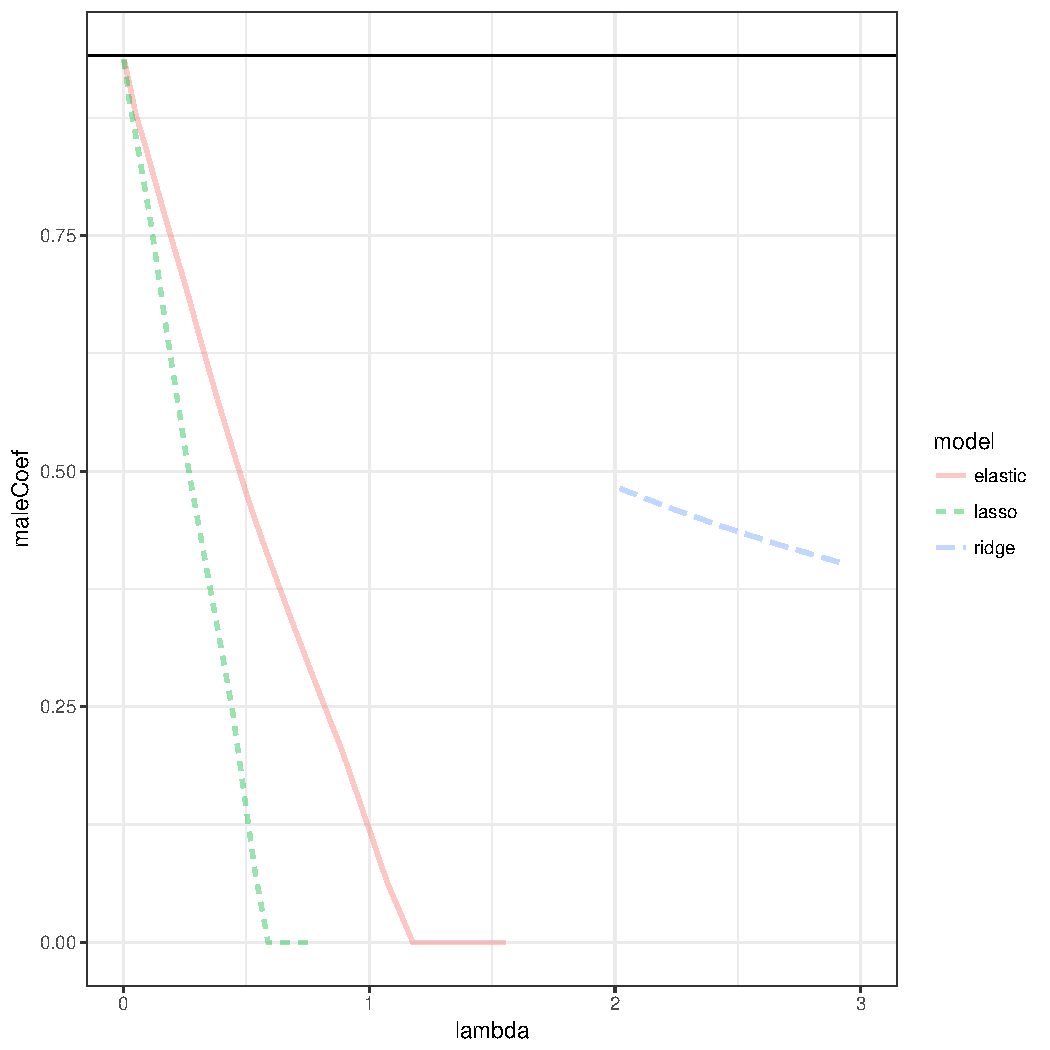
\includegraphics[width=.7\linewidth]{HW4lambda.pdf}\\
\end{figure}
  
\section{Cross-Validation, Super Learning and Ensembles}

We're going to assess the performance of five models, an unweighted average, and a super-learning average of the methods.

\begin{itemize}
\item[i)] First, set the first 20 rows to the side for use as the validation set.
\item[ii)] We'll first estimate the (unconstrained) super learner weights.
\begin{itemize}
\item[a)] On the training data (all but the first 20 rows) perform ten fold cross validation, including (1) linear regression, (2) LASSO, (3) Ridge, (4) Elastic-Net, and (5) Random Forest.  Obtain 5 predictions for each observation in the training set, one from each observation
\item[b)] Regress the dependent variable on the out of sample prediction, (without including an intercept).
\item[c)] Store those weights as $\boldsymbol{w}$
\end{itemize}
\end{itemize}

\lstinputlisting[language=R, firstline=42, lastline=84]{WUSTL_HW4_JZ.r}  

\begin{table}[H] \centering 
  \caption{\footnotesize{Model weights from regression of alcohol on the out of sample predictions for each model.} }
  \label{} 
\begin{tabular}{@{\extracolsep{5pt}}lcc} 
\\[-1.8ex]\hline 
\hline \\[-1.8ex] 
 & Estimated coefficient ($\boldsymbol{w}$) & Std. Error \\ 
  \hline
OLS Predictions & 0.0433 & 0.0631 \\ 
Lasso Predictions & 0.1050 & 3.7391 \\ 
Ridge Predictions & -0.4370 & 0.7474 \\ 
Elastic Predictions & 0.9345 & 4.2089\\ 
Random Predictions & 0.3639 & 0.1797 \\ 
   \hline
\end{tabular}
\end{table}

\begin{itemize}
\item[iii)] Now, fit all 5 models from (ii)-(a) to the entire training data set and predict the drinking level from the validation set (the data put off to the side).
\end{itemize}

\lstinputlisting[language=R, firstline=86, lastline=112]{WUSTL_HW4_JZ.r}  

\begin{table}[H] \centering 
  \caption{\footnotesize{Predicted alcohol category by model (rounded to nearest integer).} }
  \label{} 
\begin{tabular}{@{\extracolsep{5pt}}lccccc} 
\\[-1.8ex]\hline 
\hline \\[-1.8ex] 
  \footnotesize{Alcohol (validation set)} & \footnotesize{OLS preds} & \footnotesize{Lasso preds} & \footnotesize{Ridge preds} & \footnotesize{Elastic-Net preds} & \footnotesize{Random Forest preds} \\ 
  \hline
 2 & 4 & 4 & 4 & 4 & 4 \\ 
   2 & 3 & 3 & 3 & 3 & 3 \\ 
   5 & 2 & 3 & 3 & 3 & 3 \\ 
   2 & 2 & 2 & 2 & 2 & 3 \\ 
   3 & 2 & 3 & 3 & 3 & 3 \\ 
   3 & 3 & 3 & 3 & 3 & 4 \\ 
   2 & 5 & 5 & 4 & 5 & 4 \\ 
   2 & 4 & 4 & 4 & 4 & 4 \\ 
   2 & 3 & 3 & 3 & 3 & 3 \\ 
   2 & 2 & 2 & 3 & 2 & 3 \\ 
   3 & 3 & 3 & 3 & 3 & 3 \\ 
   2 & 2 & 2 & 2 & 2 & 3 \\ 
   4 & 4 & 4 & 4 & 4 & 3 \\ 
   3 & 4 & 4 & 4 & 4 & 3 \\ 
   2 & 3 & 3 & 3 & 3 & 3 \\ 
   3 & 4 & 4 & 4 & 4 & 5 \\ 
   3 & 3 & 3 & 3 & 3 & 3 \\ 
   2 & 2 & 2 & 2 & 2 & 3 \\ 
   6 & 6 & 5 & 6 & 5 & 7 \\ 
   4 & 4 & 4 & 4 & 4 & 4 \\ 
   \hline
\end{tabular}
\end{table}

\begin{itemize}
\item[iv)]   Obtain two ensemble predictions.
\begin{itemize}
\item[a)] Take the unweighted average of the predictions from the methods
\item[b)] Take the weighted average, using the weights $\boldsymbol{w}$.
\end{itemize}
\end{itemize}

\lstinputlisting[language=R, firstline=114, lastline=120]{WUSTL_HW4_JZ.r}  

\begin{itemize}
\item[v)] You should have 7 predictions. Store those in a matrix and report the correlation between the predictions
\item[vi)] Using the average absolute difference as a loss function assess the performance of each method.  Which method performs best?  Which performs the worst?

\noindent The average absolute difference for method $k$ is defined as
\begin{eqnarray}
L(\boldsymbol{Y}, \widehat{\boldsymbol{Y}}_{k}) & = & \sum_{i=1}^{N_{\text{validation}}} \frac{|Y_{i} - \widehat{Y}_{ik}| }{ N_{\text{validation}} }\nonumber
\end{eqnarray}
where $N_{\text{validation}}$ refers to the number of observations in the validation set $\widehat{\boldsymbol{Y}}_{k}$ refers to the predictions from the $k^{\text{th}}$ method,
\end{itemize}

\lstinputlisting[language=R, firstline=121, lastline=130]{WUSTL_HW4_JZ.r}  

\begin{table}[H] \centering 
  \caption{\footnotesize{Average absolute difference for each method.} }
  \label{} 
\begin{tabular}{@{\extracolsep{5pt}}lcc} 
\\[-1.8ex]\hline 
\hline \\[-1.8ex] 
 Model & $L(\boldsymbol{Y}, \widehat{\boldsymbol{Y}}_{k})$ \\ 
  \hline
OLS  & 0.838 \\ 
Lasso  & 0.847 \\ 
Ridge  & 0.836  \\ 
Elastic-Net & 0.845\\ 
Random Forest & 0.999 \\
Unweighted model average & 0.7\\
Weighted model average & 0.7\\ 
   \hline
\end{tabular}
\end{table}

\end{document}